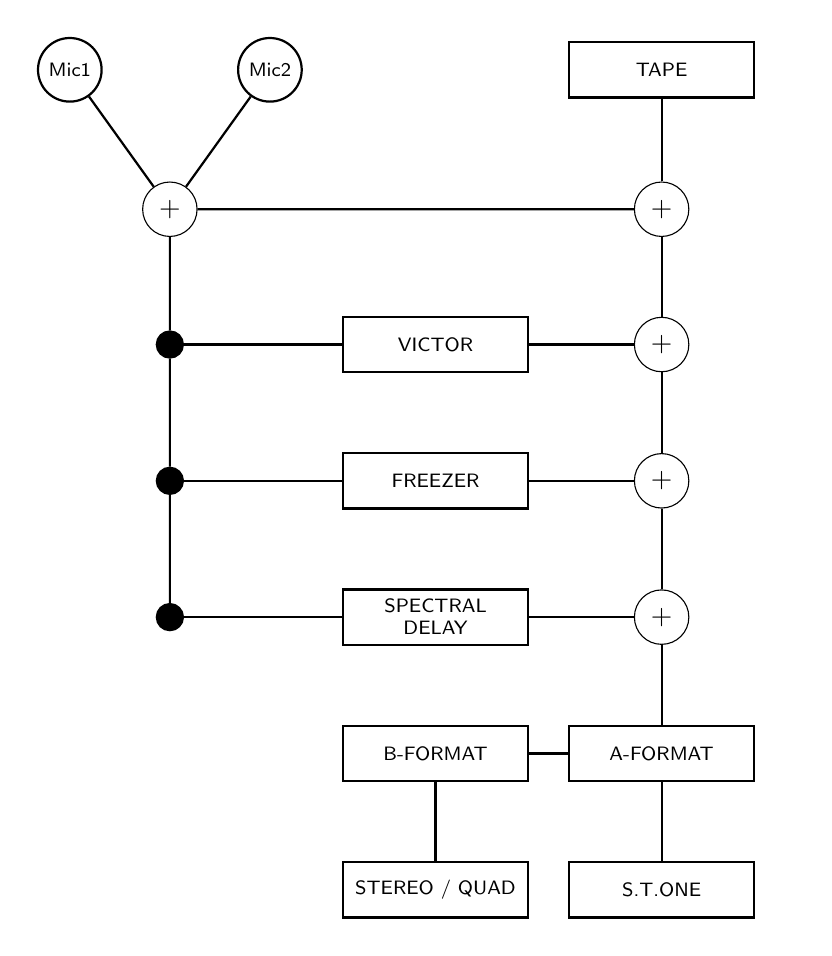
\begin{tikzpicture} [
    auto,
    mic/.style = {
    	font=\scriptsize\sffamily,
		circle,
		draw=black,
    	thick,
    	%fill=blue!20,
    	text width=2em,
    	text badly centered,
    	inner sep=1pt,
	},
    block/.style    = {
    	font=\scriptsize\sffamily,
    	rectangle,
		draw=black,
		thick,
		%fill=black!10,
		text width=6em,
		text centered,
		%rounded corners,
		minimum height=2em
		},
	line/.style = {
    	draw,
		thick,
		fill=black
		%shorten >=2pt
		},
	control/.style = {
    	draw,
		circle,
		thick,
		fill=black,
		%shorten >=2pt
		},
    arrow/.style = {
    	draw,
		thick,
		->,
		shorten >=2pt
		},
  ]
  % Define nodes in a matrix
  \matrix [column sep=5mm, row sep=10mm] {
	\node [mic] (mic1) {Mic1}; & \node [] (null1) {}; & \node [mic] (mic2) {Mic2}; & & \node [block] (tape) {TAPE}; & \\
	& \node [draw,circle] (inputs) {+}; & & & \node [draw,circle] (direct) {+}; & \\
	& \node [control] (node1) {}; & & \node [block] (victor) {VICTOR}; & \node [draw,circle] (mix1) {+}; & \\
	& \node [control] (node2) {}; & & \node [block] (freezer) {FREEZER}; & \node [draw,circle] (mix2) {+}; & \\
	& \node [control] (node3) {}; & & \node [block] (sdelay) {SPECTRAL DELAY}; & \node [draw,circle] (mix3) {+}; & \\
	& & & \node [block] (bfmt) {B-FORMAT}; & \node [block] (afmt) {A-FORMAT}; & \\
	& & & \node [block] (outputs) {STEREO / QUAD}; & \node [block] (stone) {S.T.ONE}; & \\
  };

  \begin{scope} [every path/.style=line]
  	\path (mic1) -- (inputs) -- (node1) -- (node2) -- (node3);
	\path (mic2) -- (inputs) -- (direct);
    \path (node1) -- (victor) -- (mix1);
    \path (node2) -- (freezer) -- (mix2);
    \path (node3) -- (sdelay) -- (mix3);
    \path (tape) -- (direct) -- (mix1) -- (mix2) -- (mix3);
    \path (mix3) -- (afmt) -- (stone);
    \path (afmt) -- (bfmt) -- (outputs);

  \end{scope}

\end{tikzpicture}
